\newpage
\section{Ряды Лорана, их области сходимости. Теоремы о разложении голоморфной функции и о единственности разложения в ряд Лорана. Неравенство Коши для коэффициентов ряда Лорана.}

Ряд Лорана:
$$
\sum\limits_{n=-\infty}^{+\infty} c_n(z-a)^n = \sum\limits_{n=-1}^{-\infty}c_n(z-a)^n + \sum\limits_{n=0}^{\infty}c_n(z-a)^n
$$

Первая сумма, с отрицательными коэффициентами,\\ $\sum\limits_{n=-1}^{-\infty}c_n(z-a)^n$, называется \textbf{главной частью}.

Вторая сумма называется \textbf{правильной частью}.

Ряд Лорана сходится, когда сходятся оба ряда.

Ясно, что правильная часть сходится, если  
$$|z - a| < R_1$$
где $R$ -- некоторое действительное число.
Аналогичным образом при замене $\xi = \frac{1}{z - a}$ главная часть преобразуется к обычному ряду
$$
\sum\limits_{n=-1}^{-\infty}c_n\xi^{-n}=\sum\limits_{k=1}^{\infty}c_{-k}\xi^{k}
$$
откуда $\xi<R_2$, где $R_2$ -- некоторое действительное число, откуда
$$|z - a| > R_2$$

Таким образом получаем два условия сходимости ряда Лорана, оба из которых должны выполняться для сходимости ряда, а значит областью сходимости ряда Лорана (за исключением граничных случаев) является кольцо:

\begin{center}
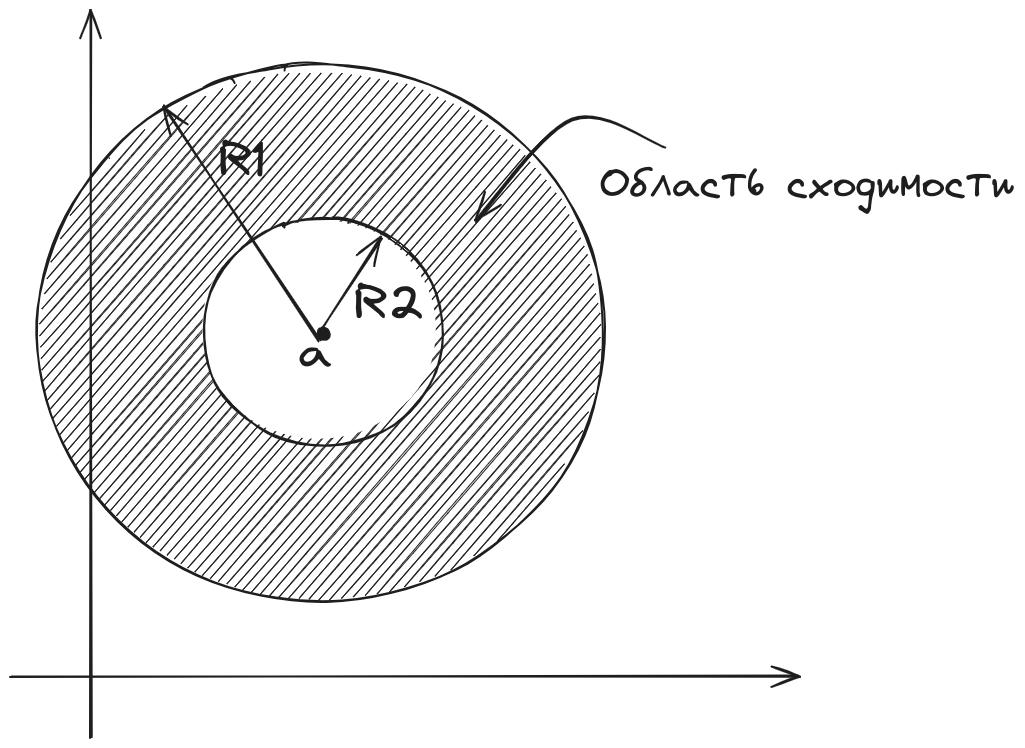
\includegraphics[scale=0.3]{answers/img/rng.png}
\end{center}

\textbf{Теорема Лорана}.\\[2mm]
Пусть $0\le R_2 < R_1 \le \infty$, $V = \{z\in\mathbb{C} ~~|~~ R_2 < |z - a| < R_1\}, f\in H(V)$.

Тогда $f(z) = \sum\limits_{-\infty}^{+\infty}c_n (z - a)^n$, где
$$
c_n = \frac{1}{2\pi i}\oint\limits_{|z - a| = \rho} \frac{f(\xi)}{(\xi - a)^{n + 1}} d\xi
$$
$n\in\mathbb{Z}, R_2 < \rho < R_1$

\begin{proof}
    \ \\
    
    \begin{figure}[h]
        \centering
        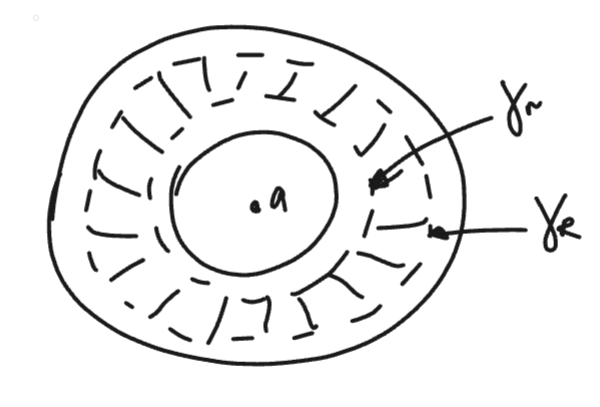
\includegraphics[width=0.4\linewidth]{answers/img/ans14.png}
    \end{figure}
    Пусть $r, R$ -- такие, что $R_2<r<R<R_1$.\\
    Тогда $V'=\{z\in \mathbb{C}: r<|z-a|<R\}$\\
    $\gamma V'=\gamma_r(a)\cup \gamma_R(a)\subset V, a\in V'$\\
    Интегральная формула Коши: $f(z)=\frac{1}{2\pi i}\cdot \int\limits_{\partial V'}\frac{f(\xi)}{\xi-z}d\xi = \frac{1}{2\pi i}\oint\limits_{\gamma_R(a)}...-\frac{1}{2\pi i}\oint\limits_{\gamma_r(a)}... (=)$\\
    На $\gamma_R(a)$ обход против часовой стрелки:\\
    $\frac{1}{\xi-z}=\frac{1}{(\xi-a)(1-\frac{z-a}{\xi-a})}=\sum_{n=0}^\infty \frac{(z-a)^n}{(\xi-a)^{n+1}}$\\ 
    На $\gamma_r(a)$ обход по часовой стрелке:\\ 
    $\frac{1}{\xi - z} = \frac{1}{(\xi-a)-(z-a)}=\frac{-1}{(z-a)(1-\frac{\xi-a}{z-a})}=$ \\
    $=-\frac{1}{z-a}\sum_{n=0}^\infty \frac{(\xi-a)^n}{(z-a)^n}=-\sum_{n=0}^\infty \frac{(\xi-a)^n}{(z-a)^{n+1}} = -\sum_{k=-1}^{-\infty} \frac{(z-a)^k}{(\xi-a)^{k+1}}$\\
    Тогда:\\
    $(=) \sum_{n=0}^{+\infty} \frac{1}{2\pi i} \oint\limits_{\gamma_R(a)}f(\xi) \frac{(z-a)^n}{(\xi-a)^{n+1}}d\xi \ +$\\
    $+\sum_{k=-1}^{-\infty}\frac{1}{2\pi i}\cdot \oint\limits_{\gamma_r(a)}f(\xi)\frac{(z-a)^k}{(\xi-a)^{k+1}}d\xi=$ \\
    $= \sum\limits_{n=0}^{+\infty} c_n(z-a)^n+\sum_{k=-1}^{-\infty}c_k(z-a)^{-k}$ 
    
\end{proof}

\textbf{Теорема о единственности разложения в ряд Лорана.}\\[2mm]
Если в кольце $V = \{z\in\mathbb{C} ~~|~~ r < |z - a| < R\}$
$$
(*) f(z) = \sum\limits_{n=-\infty}^{+\infty}c_n(z - a)^n
$$
то
$$
c_n = \frac{1}{2\pi i}\oint\limits_{|z - a| = \rho} \frac{f(\xi)}{(\xi - a)^{n + 1}} d\xi
$$
где $n\in\mathbb{Z}, r < \rho < R$

\begin{proof}
    \ \\
    Ряд сходится равномерно на $\gamma$, т.к.:\\
    $f(z)=\sum_{n=0}^\infty c_n(z-a)^n + \sum_{k=1}^\infty c_{-k}(z-a)^{-k}$\\
    1.\\
    $|c_n(z-a)^n|=|c_n|\cdot|z-a|^n=|c_n|\rho^n < |c_n|R^n, z=a+\rho e^{it}$\\
    $r<r_1<\rho<R_1<R$\\
    $\sum|c_n|R^n$ -- сходится, значит по признаку Вейерштрасса первая часть  $f(z)$ сходится равномерно.\\
    2.\\
    $|c_{-k}(z-a)^{-k}|=\frac{|c_{-k}|}{|z-a|^k}=\frac{|c_{-k}|}{\rho^k}<\frac{|c_{-k}|}{r_1^k}$;\\
    $\sum \frac{|c_{-k}}{r_1^k}$ сходится, значит вторая часть сходится равномерно.\\[2mm]
    $f(z)\cdot (z-a)^{-k-1}=\sum_{n=-\infty}^\infty c_n(z-a)^{n-k-1}\Rightarrow \oint\limits_{\gamma}\frac{f(z)}{(z-a)^{k+1}}dz=\sum_{n=-\infty}^{+\infty}c_n\oint\limits_{\gamma}(z-a)^{n-k-1}dz = 
    \begin{cases}
        0,\text{ если }n-k\neq 0\\
        2\pi i\text{, если }n-k=0
    \end{cases}
    =c_k \cdot 2\pi i$

\end{proof}

\textbf{Неравенство Коши для коэффициентов Лорана.}\\[2mm]
Пусть $V = \{z\in\mathbb{C} ~~|~~ r < |z - a| < R\}$, $f\in H(V)$, \\$\gamma = \{z ~~ : ~~ |z - a| = \rho\}, \rho\in(r,R)$\\
$\forall z\in\gamma~~ |f(z)|\le M$, тогда
$$
|c_n| \le \frac{M}{\rho^n}, \forall n\in\mathbb{Z}
$$
